\documentclass[10pt,a4paper]{article}
\usepackage[utf8]{inputenc}
\usepackage[spanish]{babel}
\usepackage{amsmath}
\usepackage{amsfonts}
\usepackage{amssymb}
\usepackage{graphicx}
\author{Carlos Manuel Rodríguez Martínez}
\title{Proyecto máquina de Turing}
\begin{document}

\section{Introducción}

\section{Máquina de Turing}

\subsection{Definición formal de máquina de Turing}

Formalmente se define a una máquina de Turing como una 7-tupla, $(Q,\Sigma, \Gamma, \delta, q_0, q_{\text{aceptar}},q_{\text{rechazar}})$, donde $Q$, $\Sigma$, $\Gamma$ son conjuntos finitos, y
\begin{enumerate}
	\item $Q$ es el conjunto de estados,
	\item $\Sigma$ es el alfabeto de entrada que no contiene el \textbf{símbolo vacío} \textvisiblespace,
	\item $\Gamma$ es el alfabeto de la cinta, donde $\textvisiblespace \in \Gamma$ y $\Sigma \subseteq \Gamma$,
	\item $\delta : Q \times \Gamma \rightarrow Q \times \Gamma \times \{ L, R \}$ es la función de transición,
	\item $q_0 \in Q$ es el estado inicial,
	\item $q_{\text{aceptar}} \in Q$ es el estado de aceptación, y
	\item $q_{\text{rechazar}} \in Q$ es el estado de rechazo, donde $q_{\text{rechazar}} \neq q_{\text{aceptar}}$.
\end{enumerate}

Esta definición implica la existencia de una configuración de símbolos de la cinta que es específica para cada instante del cómputo que realiza la máquina, junto con el estado asociado a cada configuración y la posición de la cabeza lectora de la máquina. Esta configuración puede representarse por la cadena $u \, q \, v$, donde $u, v \in \Gamma$ son cadenas, y $q \in Q$ es un estado.

Por ejemplo, para una máquina de Turing cuya cinta tiene la cadena $101101111$, se encuentra en el estado $q_7$ y la cabeza se ubica en la posición $4$, esto es sobre el segundo cero, identificando a $u$, y $v$ como $1011$ y $01111$ respectivamente,
\[	
\overbrace{ \underbrace{1011}_\text{u} \underbrace{01111}_\text{v}}^\text{cinta}
\]
la configuración se codifica como $1011q_7 01111$.
Se dice que una máquina de Turing con una configuración $C_1$ produce $C_2$ si se puede transitar de $C_1$ a $C_2$ en un solo paso. Más formalmente, sea $a, b, c \in \Gamma$, $u, v \in \Gamma^*$, y estados $q_i, q_j \in Q$. Sean $u a q_i b v$ y $u q_j a c v$ dos configuraciones,
\[
	u a q_i b v \rightarrow u q_j a c v
\]
sii la función de transición es $\delta(q_i, b) = (q_j, c, L)$. Asimismo,
\[
	u a q_i b v \rightarrow u a c q_j v
\]
sii la función de transición es $\delta(q_i, b) = (q_j, c, R)$.

Existen configuraciones especiales de la máquina donde es relevante hacer una distinción. Sea $M$ una máquina de Turing, que actúa sobre una entrada $w$, se define que:

\begin{itemize}
	\item su \textbf{configuración inicial} es $q_0 w$,
	\item su \textbf{configuracion de aceptación} es una cuyo estado sea $q_{\text{aceptar}}$,
	\item su \textbf{configuración de rechazo} es una cuyo estado sea $q_{\text{rechazar}}$,
	\item su \textbf{configuración de interrupción} es o bien una configuración de aceptación o de rechazo.
\end{itemize}

Se dice que $M$ \textbf{acepta} una entrada $w$ si existe una secuencia de configuraciones $C_1, C_2, \dots, C_k$ donde:
\begin{enumerate}
	\item $C_1$ es la configuración inicial de $M$ en  la entrada $w$,
	\item cada $C_i$ produce $C_{i+1}$, y
	\item $C_k$ es una configuración de aceptación.
\end{enumerate}

\subsection{Codificación de Penrose}
\subsubsection{Descripción del programa}
La codificación de Penrose es una manera de asignar un número natural a cada posible máquina de Turing. Para esto se restringe el alfabeto de entrada a un sólo símbolo, de manera que el alfabeto de la cinta es $\Gamma = \{0,1\}$ donde se toma al $0$ como símbolo vacío. Se establece la siguiente notación para la descripción de un programa:
\[
	_{q_i}\textbf{R} \rightarrow _{q_j}\textbf{W}_{D},
\]
donde $q_i$ es el estado de la configuración $i$, $\textbf{R}$ es el símbolo que lee la máquina, $q_j$ es el estado de la configuración $j$, $\textbf{W}$ es el símbolo que escribe la máquina y $D$ es la dirección que puede ser $D = \{L,R\}$. La descripción de un programa se da por medio de la concatenación de instrucciones, por ejemplo:

\begin{align*}
	&_{0}\textbf{0} \rightarrow _{0}\textbf{0}_{R} \\
	&_{0}\textbf{1} \rightarrow _{13}\textbf{1}_{L} \\
	&_{1}\textbf{0} \rightarrow _{65}\textbf{1}_{R} \\
	&_{1}\textbf{1} \rightarrow _{1}\textbf{0}_{R} \\
	&_{2}\textbf{0} \rightarrow _{0}\textbf{1}_{Halt} \\
	&_{2}\textbf{1} \rightarrow _{66}\textbf{1}_{L} \\
	& \vdots \\
	&_{258}\textbf{1} \rightarrow _{0}\textbf{0}_{Halt} \\
	&_{259}\textbf{0} \rightarrow _{97}\textbf{1}_{R} \\
	&_{259}\textbf{1} \rightarrow _{0}\textbf{0}_{Halt}
\end{align*}

Esta notación para la descripción de un programa resulta conveniente para la lectura humana en la interpretación de un algoritmo, sin embargo si lo que se busca es la notación más compacta es posible hacer varias mejoras.

Primero, la información de la columna izquierda es redundante, la posición de cada instrucción es suficiente para determinar a qué estado y símbolo corresponde. Podemos expresar el programa de la siguiente manera;
\[
	_{0}\textbf{0}_{R}, _{13}\textbf{1}_{L}, _{65}\textbf{1}_{R}, _{1}\textbf{0}_{R}, \dots, _{97}\textbf{1}_{R}, _{0}\textbf{0}_{Halt}.
\]
Se puede notar también que las comas y la notación $_{x}y_z$ son innecesarias, incluso sin ellas es posible distinguir los estados de los símbolos de entrada sin señalamiento adicional debido a que los símbolos de entrada siempre son seguidos por  L,R, o H.
\[
	0 \textbf{0} R 13 \textbf{1} L 65 \textbf{1} R 1 \textbf{0} R \dots 97 \textbf{1} R 0 \textbf{0} H
\]

Si deseamos restringir la cantidad de símbolos utilizados en la descripción de un programa podemos hacer el uso de la codificación binaria para los estados
\[
	_{0}\textbf{0}_{R}, _{1101}\textbf{1}_{L}, _{1000001}\textbf{1}_{R}, _{1}\textbf{0}_{R}, \dots, _{1100001}\textbf{1}_{R}, _{0}\textbf{0}_{Halt}
\]
o en forma más compacta
\[
	0 \textbf{0} R \quad 1101 \textbf{1} L \quad 1000001 \textbf{1} R \quad 1 \textbf{0} R \quad \dots \quad 1100001 \textbf{1} R \quad 0 \textbf{0} H
\]

Es posible simplificar esta representación quitando todos los dígitos innecesarios. Por ejemplo, $0 \textbf{0}$ se puede omitir por completo sin perder información y $0 \textbf{1}$ es posible dejarlo sólo como $1$. También, por definición de la notación utilizada, toda máquina de Turing comienza con una instrucción que mueve la cabeza lectora hacia la derecha. Es posible omitir este símbolo. Aquí se está asumiendo que todas las máquinas de Turing comienzan con la instrucción $0 \textbf{0} R$, esto asegura que el dispositivo puede empezar a funcionar arbitrariamente lejos hacia la izquierda y llegará siempre a la primera sobre la cinta.
\[
	1101 \textbf{1} L \quad 1000001 \textbf{1} R \quad 1 \textbf{0} R \quad \dots \quad 1100001 \textbf{1} R \quad H
\]
A este procedimiento que codifica el programa en la menor cantidad de símbolos se le llamará \textit{simplificación}.

A partir de la simplificación anterior, es posible codificar esta secuencia el sólo dos símbolos $\{0,1\}$ por medio de la siguiente regla de sustitución
\begin{align*}
	&0 \rightarrow 0,\\
	&1 \rightarrow 10,\\
	&R \rightarrow 110,\\
	&L \rightarrow 1110,\\
	&H \rightarrow 11110.
\end{align*}

El motivo de esta forma de codificación tiene origen en la entropía de la información. Bajo la suposición de que la cinta comienza con un número infinito de ceros que representan espacios vacíos y se mueve inicialmente hacia la derecha, es de esperar que los espacios vacíos $0$ sean más frecuentes en la cinta que las marcas $1$, asimismo el símbolo $R$ será más frecuente que $L$. Es por esto que en la codificación anterior se utiliza menor cantidad de dígitos para describir a los símbolos más frecuentes y viceversa. Esto nos asegura que la codificación minimice la entropía de la información.

Aplicando esta codificación a los símbolos no numéricos de la secuencia anterior queda lo siguiente, donde los dígitos se han encerrado entre paréntesis:
\[
	(1101) \; (1) \; 1110 \; (1000001) \; (1) \; 110 \; (1) \; (0) \; 110 \; \dots \; (1100001) \; (1) \; 110 \; 11110
\]
Aplicando la codificación a los dígitos queda terminada la segunda parte del proceso que se denomina \textit{expansión}.
\[
	101001010111010000001010110100110 \dots 10100000101011011110
\]
Por último, se puede borrar el $110$ final de la secuencia ya que siempre termina con los símbolos $L$, $R$ o $H$, que también terminan en $110$. A este tercer paso se le llama \textit{corte}.
\[
	101001010111010000001010110100110 \dots 10100000101011011
\]
El número $n$ resultante de este proceso es el número natural asociado con la máquina de Turing $T_n$.

\subsubsection{Descripción de los datos numéricos (codificación en cinta)}


\subsection{Representación de Wolfram}
Una forma alternativa de representar cada configuración de la máquina consiste en representar cada estado con una flecha y cada elemento de celda por un color. Esto nos daría que la representación equivalente de la configuración $1011q_7 01111$ es:
\begin{figure}[h!tb!]
	\centering
	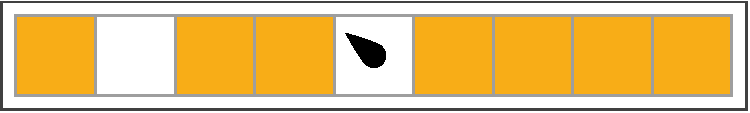
\includegraphics[scale=0.38]{figures/example_initial.pdf}
\end{figure}

Esta representación fue la utilizada por Wolfram en su libro ANKS. La ventaja de utilizar esta representación es que nos permite obtener una intuición rápida de las reglas que definen a la máquina de Turing. Por ejemplo, podemos definir a la máquina de Turing de $7$ estados y con número $213647987049278949$ de la siguiente manera:
\begin{figure}[h!tb!]
	\centering
	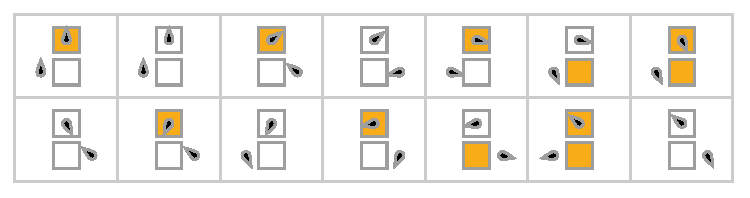
\includegraphics[scale=0.68]{figures/example_rules.pdf}
\end{figure}
cuya descripción en la notación usual es

\begin{align*}
	_{0}\textbf{0} \rightarrow _{0}\textbf{0}_L
\end{align*}

\begin{figure}[h!tb!]
	\centering
	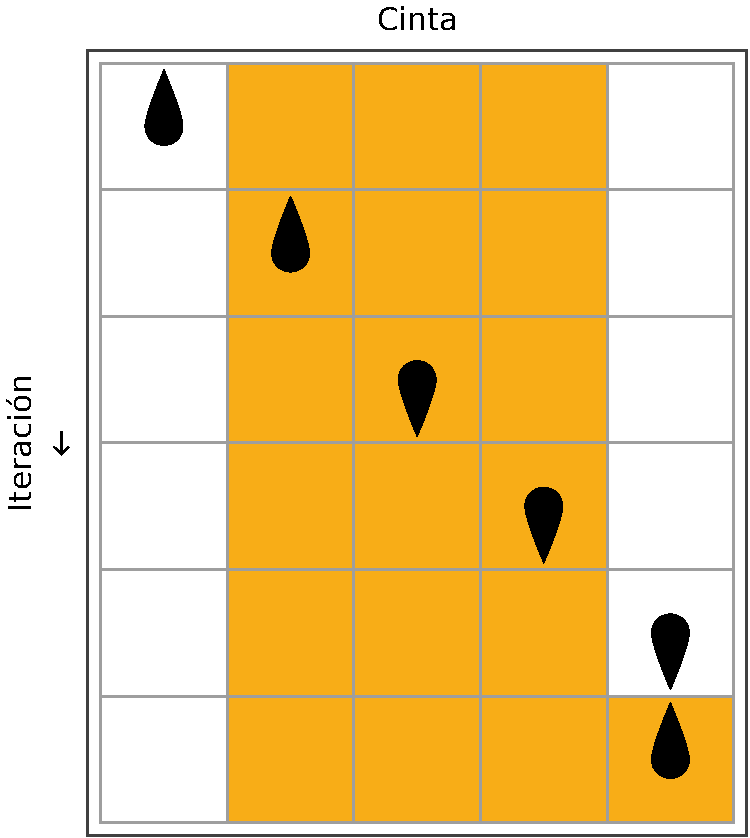
\includegraphics[scale=0.48]{figures/example_evolution.pdf}
\end{figure}

\end{document}